\documentclass{article}

\usepackage{amsmath}
\usepackage{amssymb}
\usepackage{color}
\usepackage{graphicx}
\usepackage[alsoload=binary]{siunitx}
\usepackage{booktabs}
\usepackage{multirow}
\usepackage{fancyvrb}
\usepackage[section]{placeins}
\usepackage{flafter}
\usepackage{url}
\usepackage{hyperref}

% a bit more compact
\let\l\left
\let\r\right

% no section numbers
\setcounter{secnumdepth}{-2}

% from amssymb.sty
\let\emtpyset\varnothing

% leave notes to yourself
\newcommand\todo[1]{\textcolor{red}\textsc{todo}: #1}

% write in code
\DefineShortVerb{\|}

\newcommand\figsize{.9\linewidth}

\newcommand\prot[1]{\textsc{#1}}
\newcommand\MI{\prot{mi}\xspace}
\newcommand\MSI{\prot{msi}\xspace}
\newcommand\MOSI{\prot{mosi}\xspace}
\newcommand\MESI{\prot{mesi}\xspace}
\newcommand\MOESI{\prot{moesi}\xspace}
\newcommand\MOESIF{\prot{moesif}\xspace}

\title{CS 6290 Project 3: Cache Coherence}
\author{Sam Britt}
\date{\today}

\begin{document}
  \maketitle

  \section{Results}
  \label{sec:results}
  Figure~\ref{fig:runtime} shows the runtime (in clock cycles) of the
  trace simulations for each cache coherency protocol. Because of the
  order of magnitude difference in runtime, the longer traces used for
  validation are plotted on the left, and the eight shorter traces are
  plotted separately on the right. (All results will be presented this
  way).

  Figures~\ref{fig:misses} and \ref{fig:transfers} show the number of
  cache misses and cache-to-cache transfers, respectively, that
  occurred during the simulation of each trace for each coherency
  protocol. Figure~\ref{fig:upgrades} shows, for each trace, the
  number of silent upgrades from the exclusive to the modified state.
  Data from only those protocols that have an exclusive state, namely
  \MESI, \MOESI, and \MOESIF, are shown.

  \begin{figure}[htbp]
    \label{fig:runtime}
    \centering
    \begin{minipage}[t]{\figsize}
      \centering
      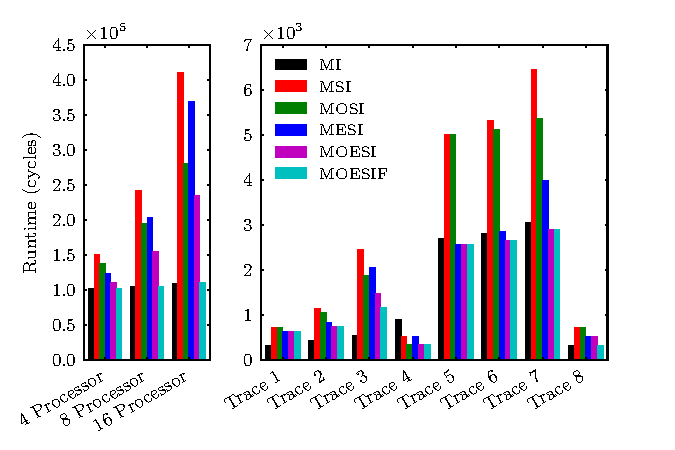
\includegraphics[width=\linewidth]{../runs/plots/runtime}
      \caption{Runtime (in clock cycles) of the various trace
        simulations using each cache coherency protocol. The longer
        validation runs are on the left plot, and the short traces are
        on the right.}
    \end{minipage}
  \end{figure}

  \begin{figure}[htbp]
    \label{fig:misses}
    \centering
    \begin{minipage}[t]{\figsize}
      \centering
      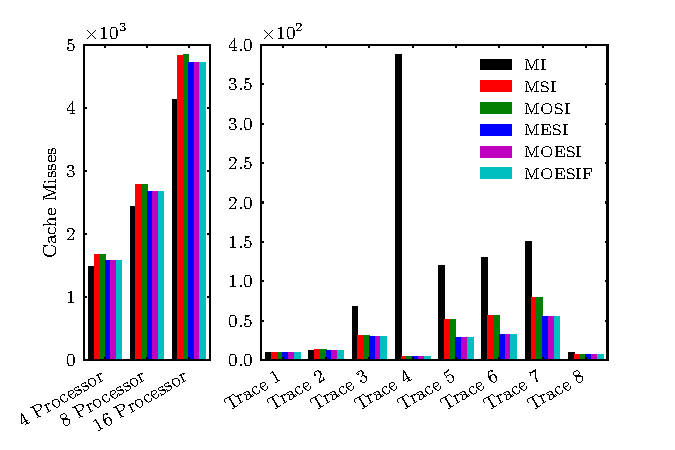
\includegraphics[width=\linewidth]{../runs/plots/misses}
      \caption{Number of cache misses during simulation of the various
        traces using each cache coherency protocol.}
    \end{minipage}
  \end{figure}

  \begin{figure}[htbp]
    \label{fig:transfers}
    \centering
    \begin{minipage}[t]{\figsize}
      \centering
      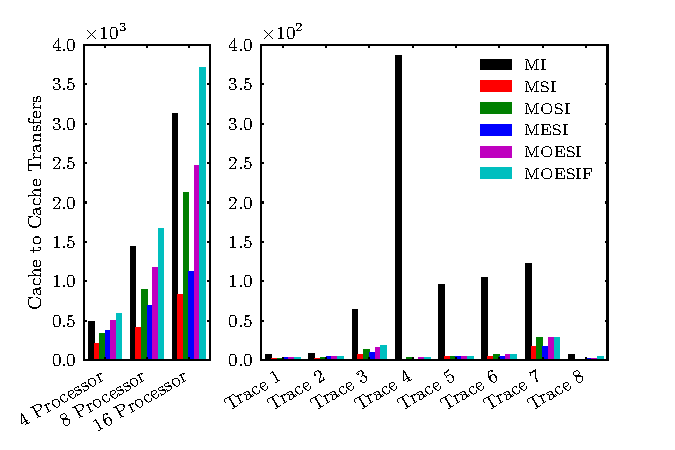
\includegraphics[width=\linewidth]{../runs/plots/transfers}
      \caption{Number of cache-to-cache transfers during simulation of
        the various traces using each cache coherency protocol.}
    \end{minipage}
  \end{figure}

  \begin{figure}[htbp]
    \label{fig:upgrades}
    \centering
    \begin{minipage}[t]{\figsize}
      \centering
      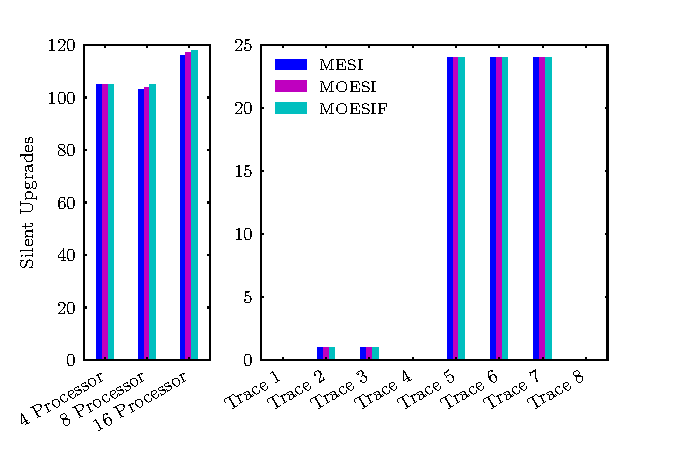
\includegraphics[width=\linewidth]{../runs/plots/upgrades}
      \caption{Number of silent upgrades to the modified state from
        the exclusive state during simulation of the various traces
        using each cache coherency protocol that contains an exclusive
        state.}
    \end{minipage}
  \end{figure}

  % section results (end)

  \section{Discussion}
  \label{sec:discussion}

  Interestingly, the simple \MI protocol outperforms most or all
  other protocols in almost every trace, as can be seen from
  Figure~\ref{fig:runtime}. Compare with the runtime results for the
  \MSI protocol: with the exception of trace $4$ (which will be
  discussed later), adding the shared state to the protocol increases
  runtime by a factor of as much as $4$. This is perhaps not as
  expected, since adding a shared state allows multiple caches to keep
  read-only copies of data, which should reduce the number of cache
  misses; indeed this is the case, as shown by
  Figure~\ref{fig:misses}. In every simulation of the short traces,
  the number of cache misses is reduced by sharing; the effect is
  particularly evident for the read-heavy traces $3$--$7$.

  However, adding the shared state removes one critical characteristic
  of the simpler \MI protocol: the high degree of cache-to-cache
  transfers.  Even if a processor needs only read-only accesses of a
  cache line, in the \MI protocol it still must be put in the modified
  state. It therefore will supply the data over the bus on the next
  request, avoiding the costly trip to memory. The effect is quite
  clearly shown by Figure~\ref{fig:transfers}. The \MI protocol may
  not allow true sharing, but sharing may not be necessary for
  performance if the bus has sufficiently low latency.

  One interesting trace is trace $4$. It seems to buck the trend: the
  \MSI protocol outperforms the \MI protocol, and the number of cache
  misses and cache-to-cache transfers using the \MI protocol dominate
  all the other traces and protocols. Upon inspection of the trace
  itself the reason became apparent. Trace $4$ simulates a machine
  with four processors. After an initial write to a particular memory
  address by the first processor, all accesses from all processors are
  reads to that address. Clearly, such an access pattern benefits from
  the sharing provided by the \MSI protocol. The penalty of going to
  memory is avoided because, after the initial access from each
  processor, the data in the cache is clean and can be provided to the
  processor directly---no need for bus or memory interaction.

  Though most traces perform well in the \MOESI and \MOESIF protocols,
  traces $5$, $6$, and $7$ seem to particularly benefit from the
  addition of the exclusive state. A quick look at
  Figure~\ref{fig:upgrades} shows the reason: the access patterns of
  those traces allow for a larger number of silent upgrades from the
  exclusive state to the modified state. This reduces the number of
  cache misses (see Figure~\ref{fig:misses}) because, without the
  exclusive state, such a cache line would be in the shared state and
  would have to go to the bus to get modified access.

  % section discussion (end)

  \section{Conclusion}
  \label{sec:conclusion}

  Based on the results of the simulations, there is little reason to
  use anything other than the \MI cache coherency protocol. In many
  cases, adding complexity to the protocol hurt performance, and in
  the other cases, the improvement in performance was not so much to
  overwhelm the increase in cost and complexity of the implementing
  the other protocols. The success of the \MI protocol, though, is
  largely due to the high discrepancy between the bus and memory
  controller latencies. If that gap were closed (by perhaps a faster
  memory controller, a slower bus), or if there were many more
  processors contending for the bus, the simpler protocol may not be
  sufficient. Also, if the memory access pattern is known \emph{a
    priori} to be, say almost exclusively read-only, a protocol with
  increased sharing may be chosen that optimizes for that use case.

  % section conclusion (end)


\end{document}
